\part{Recursion}
\label{recurs}\mypartpage
\begin{Coupe}
\section{Introduction}
%%%%%%%%%%%%%%%%%%%%%%%%%%%%%%%%%%%%%%%%%%%%%%%%%%%%%%%%%%%%%%%%%%%%%%%%%%%%%% 
\begin{frame}{Divide \& Conquer}
  \vspace{-.5\baselineskip}
  \begin{block}{Classical Algorithmic Pattern}
    \begin{itemize}
    \item When the problem is too complex to be solved directly, decompose it
    \end{itemize}
  \end{block}

  \begin{block}{When/How is it applicable?}
    \begin{enumerate}
    \item \structure{Divide:} Decompose problem into (simpler/smaller)
      sub-problems
    \item \structure{Conquer:} Solve sub-problems
    \item \structure{Glue:} Combine solutions of sub-problems
      to a solution as a whole
    \end{enumerate}
  \end{block}\medskip

  \vspace{-6.5\baselineskip}~\hfill{\includegraphics[scale=.8]{fig/rec_divide_conquer.fig}}~~~~~

  \smallskip
  \begin{boitequote}{Martin Luther King}%
    You don't have to see the whole staircase, just take the first step.
  \end{boitequote}
  
\end{frame}

%%%%%%%%%%%%%%%%%%%%%%%%%%%%%%%%%%%%%%%%%%%%%%%%%%%%%%%%%%%%%%%%%%%%%%%%%%%%%% 
\begin{frame}{Recursion}
  \visible<+->{\concept{Divide \& Conquer + sub-problems similar to big one}}
  \medskip

  \begin{block}<+->{Recursive object}
    \begin{itemize}
    \item \alert{Defined using itself}
    \item<+-> \structure{Examples}:
      \begin{itemize}
      \item $\alert{U}(n)=3\times \alert{U}(n-1)+1$ ; 
        \only<-3>{$\alert{U}(0)=1$}%
        \only<4| handout:0>{\underline{$\alert{U}(0)=1$}}
      \item Char \alert{string} = either a char followed by a \alert{string},
        or  \only<-3>{empty string}\only<4| handout:0>{\underline{empty
            string}} 
      \end{itemize}
    \item<.-> Often possible to rewrite the object, in a non-recursive way
      {\small(said \textit{iterative way})}
      \medskip
    \end{itemize}
  \end{block}

  \begin{block}<+->{Base case(s)}
    \begin{itemize}
    \item Trivial cases that can be solved directly
    \item Avoids infinite loop
    \end{itemize}
  \end{block}
\end{frame}
%%%%%%%%%%%%%%%%%%%%%%%%%%%%%%%%%%%%%%%%%%%%%%%%%%%%%%%%%%%%%%%%%%%%%%%%%%%%%% 
\begin{frame}{When the base case is missing\ldots}
  \begin{columns}
    \begin{column}{.55\linewidth}
      \begin{block}<2->{There's a Hole in the Bucket {\small(traditional)}}
        {\footnotesize%There's a hole in the bucket, dear Liza, dear Liza,\\
          There's a hole in the bucket, dear Liza, a \alert{hole}.
          
          % So fix it dear Henry, dear Henry, dear Henry,\\
          So fix it dear Henry, dear Henry, fix it.
          
          % With what should I fix it, dear Liza, dear Liza,\\
          With what should I fix it, dear Liza, with what?

          % With straw, dear Henry, dear Henry, dear Henry,\\
          With straw, dear Henry, dear Henry, with \alert{straw}.

          % But the straw is too long, dear Liza, dear Liza,\\
          The straw is too long, dear Liza, too long.
          
          % So cut it dear Henry, dear Henry, dear Henry,\\
          So cut it dear Henry, dear Henry, cut it!
          
          % With what should I cut it, dear Liza, dear Liza,\\
          With what should I cut it, dear Liza, with what?
          
          % Use the hatchet, dear Henry, dear Henry, dear Henry,\\
          Use the hatchet, dear Henry, the \alert{hatchet}.
          
          % But the hatchet's too dull, dear Liza, dear Liza,\\
          The hatchet's too dull, dear Liza, too dull.

          % So, sharpen it, dear Henry, dear Henry, dear Henry,\\
          So sharpen it dear Henry, dear Henry, sharpen it!

          % With what should I sharpen it, dear Liza, dear Liza,\\
          With what should I sharpen, dear Liza, with what?

          % Use the stone, dear Henry, dear Henry, dear Henry,\\
          Use the stone, dear Henry, dear Henry, the \alert{stone}.

          % But the stone is too dry, dear Liza, dear Liza,\\
          The stone is too dry, dear Liza, too dry.

          % So wet it, dear Henry, dear Henry, dear Henry,\\
          So wet it dear Henry, dear Henry, wet it.
          
          % With what should I wet it, dear Liza, dear Liza,\\
          With what should I wet it, dear Liza, with what?
          
          % With water, dear Henry, dear Henry, dear Henry,\\
          With water, dear Henry, dear Henry, \alert{water}.
          
          % With what should I carry it, dear Liza, dear Liza,\\
          With what should I carry it dear Liza, with what?
          
          % Use the bucket dear Henry, dear Henry, dear Henry,\\
          Use the bucket, dear Henry, dear Henry, the \alert{bucket}!
          
          % There's a hole in the bucket, dear Liza, dear Liza,\\
          There's a hole in the bucket, dear Liza, a \alert{hole}.}
      \end{block}      
    \end{column}\hspace{-2em}
    \begin{column}{.5\linewidth}
      ~\vspace{2\baselineskip}
      \begin{block}{Classical Aphorism}
        ~~~To understand \alert{recursion},\\
        ~~~you first have to understand \alert{recursion}
      \end{block}

      \begin{block}<3->{Recursive Acronyms}
        \begin{itemize}
        \item \alert{G}NU is \alert{N}ot \alert{U}nix
        \item \alert{P}HP: \alert{H}ypertext \alert{P}reprocessor
        \item \alert{P}NG's \alert{N}ot \alert{G}IF
        \item \alert{W}ine \alert{I}s \alert{N}ot an \alert{E}mulator
        \item {\small\alert{V}isa \alert{I}nternational \alert{S}ervice
            \alert{A}ssociation}
        \item {\small\underline{\alert{H}\textsc{ird}} of
            \alert{U}nix-\alert{R}eplacing \alert{D}aemons\\
            \alert{H}urd of \alert{I}nterfaces \alert{R}epresenting
            \alert{D}epth}
        \item \alert{Y}our \alert{O}wn \alert{P}ersonal \alert{Y}OPY
        \end{itemize}
      \end{block}
    \end{column}
  \end{columns}

  \bigskip This is naturally to be avoided in algorithms
\end{frame}
%%%%%%%%%%%%%%%%%%%%%%%%%%%%%%%%%%%%%%%%%%%%%%%%%%%%%%%%%%%%%%%%%%%%%%%%%%%%%% 
\begin{frame}{In Mathematics: Natural Numbers and Induction}
  \begin{block}{Peano postulates (1880)}\medskip
    Defines the set of natural integers $\mathbb{N}$
    \begin{enumerate}
    \item 0 is a natural number
    \item If $n$ is natural, its successor (noted $n+1$) also
    \item There is no number $x$ so that $x+1=0$
    \item Distinct numbers have distinct successors ($x\neq y
      \Leftrightarrow x+1\neq y+1$)
    \item If a property holds (i) for 0 (ii) for each number's successor, \\
      it then holds for any number
    \end{enumerate}
  \end{block}

  \begin{block}{Proof by Induction}
    \begin{itemize}
    \item One shows that the property holds for 0 (or other base case)
    \item One shows that \alert{when} it holds for $n$, it \alert{then} holds
      for $n+1$
    \item This shows that it holds for any number
    \end{itemize}
  \end{block}
\end{frame}
%%%%%%%%%%%%%%%%%%%%%%%%%%%%%%%%%%%%%%%%%%%%%%%%%%%%%%%%%%%%%%%%%%%%%%%%%%%%%% 
\begin{frame}{In Computer Science}

  \begin{block}{Two twin notions}
    \begin{itemize}\large
    \item \structure{Functions and procedures} defined recursively (generative
      recursion) 
    \item \structure{Data structures} defined recursively (structural recursion)
    \end{itemize}    

    Naturally, recursive functions are well fitted to recursive data structures
  \end{block}\bigskip

  \begin{block}{This is an \textbf{algorithm} characteristic}
    \begin{itemize}
    \item No problem is intrinsically recursive 
    \item Some problems \textit{easier} or more natural to solve recursively
    \item Every recursive algorithm can be \textit{derecursived}
    \end{itemize}
  \end{block}
\end{frame}
%%%%%%%%%%%%%%%%%%%%%%%%%%%%%%%%%%%%%%%%%%%%%%%%%%%%%%%%%%%%%%%%%%%%%%%%%%%%%%
\section{Principles of Recursion}
\mypartpage
%%%%%%%%%%%%%%%%%%%%%%%%%%%%%%%%%%%%%%%%%%%%%%%%%%%%%%%%%%%%%%%%%%%%%%%%%%%%%%
\subsection{First Example: Factorial}
\begin{frame}{Recursive Functions and Procedures}
  \concept{\textbf{Recursively Defined Function}: its body contains calls to itself}
  
  \bigskip

  \begin{block}{The Scrabble\texttrademark\ word game}
    \begin{itemize}
    \item Given 7 letter tiles, one should form existing English worlds

      \framebox{T} \framebox{I} \framebox{R} \framebox{N} \framebox{E}
      \framebox{G} \framebox{S} $\leadsto$ RIG, SIRE, GRINS, INSERT,
      RESTING, \ldots 

    \item How many permutation exist?
      \begin{itemize}
      \item \structure{First position:} pick one tile from 7
      \item \structure{Second position:} pick one tile from 6 remaining
      \item \structure{Third position:} pick one tile from 5 remaining
      \item ...
      \item \structure{Total:} $7\times6\times5\times4\times3\times2\times1$
      \end{itemize}
    \end{itemize}
  \end{block}

  \begin{block}{This is the Factorial}
    \begin{itemize}
    \item Mathematical definition of factorial:
      $\left\{
        \begin{array}{l}
          n! = n \times (n-1)! \\
          0! = 1
        \end{array}\right.$
      
      \item Factorial : integer $\rightarrow$ integer\\
        \structure{Precondition}: factorial(n) defined if and only if $n\geq 0$\\
        \structure{Postcondition}: factorial(n)$=n!$
    \end{itemize}
  \end{block}
\end{frame}
%%%%%%%%%%%%%%%%%%%%%%%%%%%%%%%%%%%%%%%%%%%%%%%%%%%%%%%%%%%%%%%%%%%%%%%%%%%%%%
\begin{frame}{Recursive Algorithm for Factorial}
  \concept{Literal Translation of the Mathematical Definition}
  \bigskip\bigskip

  \centerline{\fbox{\vbox{\large\vspace{-.8\baselineskip} %
    \begin{tabbing}%
    \textsc{factorial}(n):\\
      ~~\=\textbf{if} n = 0 \=\textbf{then} \=$r\leftarrow 1$ \\
      \>\> \textbf{else} \>$r\leftarrow n\times factorial(n-1)$\\
      \>\textbf{end}%
    \end{tabbing}\vspace{-.8\baselineskip}%
  }}}

\bigskip
\bigskip
Remarks:
\begin{itemize}
\item \framebox{$r\leftarrow 1$} is the \alert{base case}: no recursive call
\item \framebox{$r\leftarrow n\times factorial(n-1)$} is the \alert{general
    case}: Achieves a recursive call
\item Reaching the base case is mandatory for the algorithm to finish
\end{itemize}

\end{frame}
%%%%%%%%%%%%%%%%%%%%%%%%%%%%%%%%%%%%%%%%%%%%%%%%%%%%%%%%%%%%%%%%%%%%%%%%%%%%%%
\begin{frame}{Factorial Computation Details}
  
  \centerline{\fbox{\vbox{\vspace{-1.1\baselineskip} %
    \begin{tabbing}%
    \textsc{factorial}(n):\hspace{43mm}~\\
      ~~\=\textbf{if} n = 0 \=\textbf{then} \=\kill
      \>\textbf{if} n = 0 \>\textbf{then} \>%
      \only<1-5,7->{$r\leftarrow 1$}%
      \only<6| handout:0>{\alert{$\boldsymbol{r\leftarrow 1}$}}%
      \\
      \>\> \textbf{else} \>%
      \only<1,6->{$r\leftarrow n\times factorial(n-1)$}%
      \only<2-5| handout:0>{\alert{$\boldsymbol{r\leftarrow n\times factorial(n-1)}$}}%
      \\
      \>\textbf{end}%
    \end{tabbing}\vspace{-1.2\baselineskip}%
  }}}\medskip

  $
  \left.\begin{array}{l}
    factorial(4) = \uncover<2->{4 \times factorial(3)}\\
\uncover<3->{\qquad\qquad\qquad\qquad\overbrace{3 \times factorial(2)}}\\
\uncover<4->{\qquad\qquad\qquad\qquad\qquad\overbrace{2\times
    factorial(1)}}\\ 
\uncover<5->{\qquad\qquad\qquad\qquad\qquad\qquad\overbrace{1\times
    factorial(0)}}\\
  \end{array}\uncover<7->{\right\}}
  $\uncover<7->{ \alert{Recursive Descent}}\medskip

  $
  \left.\begin{array}{l}
      \qquad\qquad\qquad\quad \uncover<7->{4\times 3\times 2\times
        1\times}\quad
      \uncover<6->{\overbrace{1}}\qquad\:
  \end{array}\uncover<6->{\right\}}
  $ \uncover<6->{\alert{Base Case}}\medskip


  $
  \left.\begin{array}{l}
      \uncover<8->{\qquad\qquad\qquad\quad 4\times 3\times 2\times  \overbrace{\qquad 1\qquad}}\qquad\:\!\:\\
       \uncover<9->{\qquad\qquad\qquad\quad 4\times 3\times\overbrace{\qquad 2\qquad}}\\
       \uncover<10->{\qquad\qquad\qquad\quad 4\times\overbrace{\qquad 6\qquad}}\\
       \uncover<11->{\qquad\qquad\qquad\quad\overbrace{\qquad 24\qquad}}\\
  \end{array}\uncover<12->{\right\}}
  $ \uncover<12->{\alert{Recursive Climb}}\medskip

  $  \left.\begin{array}{l}
       \uncover<12->{factorial(4) = 24}
     \end{array}\right.
  $


\end{frame}
%%%%%%%%%%%%%%%%%%%%%%%%%%%%%%%%%%%%%%%%%%%%%%%%%%%%%%%%%%%%%%%%%%%%%%%%%%%%%%
\subsection{Schemas of Recursion}
\subsectionpage
\begin{frame}{General Recursion Schema}

  \centerline{\fbox{\vbox{\large\vspace{-.8\baselineskip} %
    \begin{tabbing}%
      \textbf{if} \structure{\textsc{Cond}} \=\textbf{then}
      \=\structure{\textsc{BaseCase}} \\
      \> \textbf{else} \>\structure{\textsc{GenCase}}\\
      \textbf{end}%
    \end{tabbing}\vspace{-1.1\baselineskip}%
  }}}
  \medskip

  \begin{itemize}
  \item \structure{\textsc{Cond}} is a boolean expression
  \item If \textsc{Cond} is true, execute the \alert{base case}
    \structure{\textsc{BaseCase}} 
    (\alert{without recursive call})
  \item If \textsc{Cond} is false, execute the \alert{general case}
    \structure{\textsc{GenCase}}
    (\alert{with recursive calls})
  \end{itemize}

  \begin{block}{The factorial(n) example}
    \begin{description}
    \item[\textsc{BaseCase}:] $r\leftarrow 1$
    \item[\textsc{GenCase}:] $r\leftarrow n\times factorial(n-1)$
    \end{description}
  \end{block}
\end{frame}
%%%%%%%%%%%%%%%%%%%%%%%%%%%%%%%%%%%%%%%%%%%%%%%%%%%%%%%%%%%%%%%%%%%%%%%%%%%%%%
\begin{frame}[fragile]{Other Recursion Schema: \alert{Multiple Recursion}}

\Concept{More than one recursive call}\bigskip

\begin{block}{Example: Pascal's Rule and $\left(^n_k\right)$}
  \begin{itemize}
  \item Amount of $k$-long sets of $n$ elements (order ignored)
    $$ \left(^n_k\right) = \left \{
      \begin{array}{cl}
        1 & \mbox{if } k = 0 \mbox{ or } n=k;\\
        \left(^{n-1}_{~k}\right)  +  \left(_{k-1}^{n-1}\right) & \mbox{else }
        (1\leq k<n).
      \end{array}
    \right.
    $$  
  \item \framebox{$\left(_2^4\right)=6$} $\leadsto$ 6 ways to build a pair of
    elements picked from 4 possibilities:\\[4pt]
    \{A;B\},\{A;C\},\{A;D\},\{B;C\},\{B;D\},\{C;D\}\hfill (if order matters,
    $4\times 3$ possibilities)
  \end{itemize}
\end{block}

\begin{columns}
  \begin{column}{.65\linewidth}
    \begin{block}{Corresponding Algorithm:}
      \begin{tabbing}
        au\=\kill
        \textsc{Pascal} ($n$, $k$)\\[1mm]
        \> \textbf{If} $k=0$ or $k=n$ \=\textbf{then} \=$r\leftarrow 1$\\
        \>                            \>\textbf{else} \>$r\leftarrow$
                                        \=\textsc{Pascal} ($n-1$, $k$) +\\
        \>\>\>\>\textsc{Pascal} ($n-1$, $k-1$)
      \end{tabbing}  
    \end{block}    
  \end{column}
  \begin{column}{.33\linewidth}
    \begin{Verbatim}[label=First rows]
            1
          1   1
        1   2   1
      1   3   3   1
    1   4  (6)  4   1      
  1   5   10  10  5   1      
1   6   15  20  15  6   1      
    \end{Verbatim}
  \end{column}
\end{columns}

\end{frame}
%%%%%%%%%%%%%%%%%%%%%%%%%%%%%%%%%%%%%%%%%%%%%%%%%%%%%%%%%%%%%%%%%%%%%%%%%%%%%%
\begin{frame}{Other Recursion Schema: \alert{Mutual Recursion}}

\Concept{Several functions calling each other}\bigskip

\begin{block}{Example 1}
  \begin{columns}
    \begin{column}{.4\linewidth}
      $$A(n)=\left\{
        \begin{array}{cl}
          1      &\text{ if } n\leq1\\
          B(n+2) & \text{ if } n>1
        \end{array}\right.$$  
      \end{column}
      \begin{column}{.4\linewidth}
      $$B(n)=\left\{
        \begin{array}{cl}
          1        & \text{ if } n\leq1\\
          A(n-3)+4 & \text{ if } n>1
        \end{array}\right.$$  
      \end{column}
    \end{columns}
    \medskip Compute A(5):
  \end{block}

\begin{block}{Example 2: one definition of parity}\vspace{-\baselineskip}
  $$ \mbox{\alert{even?}}(n) = \!\left \{\!%
  \begin{array}{cl}
    \mbox{\textit{true}} & \mbox{if } n = 0\\
    \mbox{\alert{odd}}(n-1) & \mbox{else}
  \end{array}
\right.
\quad \mbox{and} \quad
\mbox{\alert{odd?}}(n) = \!\left \{\!%
  \begin{array}{cl}
    \mbox{\textit{false}} & \mbox{if } n = 0\\
    \mbox{\alert{even}}(n-1) & \mbox{else}
  \end{array}
\right.
$$
\end{block}

% \begin{block}{Corresponding Algorithm:}\vspace{-.6\baselineskip}
%   \begin{columns}
%     \begin{column}{0.4\linewidth}
%       \begin{tabbing}
%         au\=\kill
%         \textsc{\alert{Even}} ($n$)\\[1mm]
%         \> \textbf{If} $n=0$ \=\textbf{then} \=return \textit{true}\\
%         \>                   \>\textbf{else} \>return  \textsc{\alert{Odd}} ($n-1$)
%       \end{tabbing}
%     \end{column}\begin{column}{0.4\linewidth}
%       \begin{tabbing}
%         au\=\kill
%         \textsc{\alert{Odd}} ($n$)\\[1mm]
%         \> \textbf{If} $n=0$ \=\textbf{then} \=return \textit{false}\\
%         \>                   \>\textbf{else} \>return  \textsc{\alert{Even}} ($n-1$)
%       \end{tabbing}
%     \end{column}
%   \end{columns}
% \end{block}\medskip

\begin{block}{Other examples}
  \begin{itemize}
  \item Some Maze Traversal Algorithm also use Mutual Recursion (see lab)
  \item Mutual Recursion classical in Context-free Grammar (see compilation course)
  \end{itemize}
\end{block}
\end{frame}
%%%%%%%%%%%%%%%%%%%%%%%%%%%%%%%%%%%%%%%%%%%%%%%%%%%%%%%%%%%%%%%%%%%%%%%%%%%%%%
\begin{frame}{Other Recursion Schema: \alert{Embedded Recursion}}

\Concept{Recursive call as Parameter}\bigskip

\begin{block}{Example: Ackerman function}
  
$$
A(m, n) = \left \{
  \begin{array}{cl}
    n + 1 & \mbox{ if } m =0\\
    A(m-1, 1) & \mbox{ if } m > 0 \mbox{ and } n = 0\\
    A(m - 1, A(m, n-1)) & \mbox{ else }
  \end{array}
\right.
$$
\end{block}\vspace{-.8\baselineskip}

\begin{block}{Thus the algorithm:}\vspace{-.8\baselineskip}
\begin{tabbing}
  au\=au\=au\=au\=\kill
  \textsc{Ackerman}($m$, $n$)\\
  \> \textbf{if} $m = 0$ \= \textbf{then} $n+1$\\
  \> \> \textbf{else if} $n = 0$ \=\textbf{then} \textsc{Ackerman}($m-1$, 1)\\
  \> \>                           \>\textbf{else} \textsc{Ackerman}\alert{(}$m-1$, \textsc{Ackerman}($m$, $n-1$)\alert{)}
\end{tabbing}
\end{block}\vspace{-.8\baselineskip}

\uncover<2->{
\begin{block}{Warning, this function grows quickly:}\smallskip
  $Ack(1,n)=n+2$\hspace{3cm}
  $Ack(2,n)=2n+3$

  $Ack(3,n)=8\cdot 2^n -3$\hspace{24mm}
  $Ack(4,n)=2^{2^{\left.2^{\ldots^2}\right\}n}}$

  $Ack(4,4)>2^{65536}>10^{80}$ (estimated amount of particles in universe)
\end{block}
}
\end{frame}
%%%%%%%%%%%%%%%%%%%%%%%%%%%%%%%%%%%%%%%%%%%%%%%%%%%%%%%%%%%%%%%%%%%%%%%%%%%%%%
\subsection{Recursive Data Structures}
%%%%%%%%%%%%%%%%%%%%%%%%%%%%%%%%%%%%%%%%%%%%%%%%%%%%%%%%%%%%%%%%%%%%%%%%%%%%%%
\begin{frame}\frametitle{Recursive Data Structures}

  \begin{alertblock}{Definition}
    \begin{description}
    \item[Recursive datatype:] Datatype defined using itself
    \end{description}
  \end{alertblock}

  \begin{block}{Classical examples}
    \begin{description}
    \item[List:] element followed by a list or empty list
    \item[Binary tree:] \{value; left son; right son\} or empty tree
    \end{description}
  \end{block}


  \begin{block}{This is the subject of the module ``Data Structures''}
    \begin{itemize}
    \item After TOP and POO in track
    \end{itemize}
  \end{block}
\end{frame}
%%%%%%%%%%%%%%%%%%%%%%%%%%%%%%%%%%%%%%%%%%%%%%%%%%%%%%%%%%%%%%%%%%%%%%%%%%%%%%
\begin{frame}\frametitle{Example: Strings as (linked) lists}

  \begin{block}{Defined operations}
    \medskip
    \begin{tabular}{l@{$\;$}l@{$\;$}l}
      \structure{[ ]} & &\textit{The empty string object}\\
      \structure{cons}&Char $\times$ String $\mapsto$ String&
      \textit{Adds the char in front of the list}\\
      \structure{car}&String $\mapsto$ Char&
        \textit{Get the first char of the list}\\
        &&\textit{\small(not defined if empty?(str))}\\
      \structure{cdr}&String $\mapsto$ String&
        \textit{Get the list without first char}\\
      \structure{empty?}& String $\mapsto$ Boolean&
        \textit{Tests if the string is empty}\\
    \end{tabular}
  \end{block}

  \begin{itemize}
  \item As you can see, strings are defined recursively using strings
  \end{itemize}

  \begin{block}{Examples}
    \begin{itemize}
    \item ``bo'' = cons('b',cons('o',[ ]))
    \item ``hello'' = 
      cons('h',cons('e',cons('l',cons(cons('l',cons(cons('o',[ ])))))))
    \item cdr(cons('b',cons('o',[ ]))) = ``o'' = cons('o',[ ])
    \end{itemize}
  \end{block}

  \begin{alertblock}{These are native constructs in LISP programing language}
  \begin{itemize}\vspace{-.3\baselineskip}
  \item But, these constructs are hard to remember (cdr vs. car)
  \item But, all these parenthesis are nasty (too much syntaxic sugar)
  \end{itemize}
  \end{alertblock}
\end{frame}
%%%%%%%%%%%%%%%%%%%%%%%%%%%%%%%%%%%%%%%%%%%%%%%%%%%%%%%%%%%%%%%%%%%%%%%%%%%%%%
\begin{frame}[fragile]\frametitle{Doing the same in Java}
  \begin{description}
  \item[Element] Class representing a letter and the string following
    (ie, non-empty strings)
  \item[String] Class representing a string (either empty or not)
  \end{description}\vspace{-.6\baselineskip}

  \begin{columns}[t]
    \begin{column}{.36\linewidth}
      \begin{boitecode}{}
public \alert{class Element} \{
  public char value;
  public Element tail;

  Element(char x, Element tail) \{
      value = x;
      this.tail = tail;
  \}    
\}
  \end{boitecode}
    \end{column}

    \begin{column}{.5\linewidth}
  \begin{boitecode}{}
public \alert{class StringRec} \{
  private Element head = null;

  public boolean isEmpty() \{ 
      return head == null;
  \}
  public void cons(char x) \{
    \structure{// Create new elem and connect it}
    Element newElem = new Element(x, head);
    \structure{// This is new head}
    head = newElem;
\} \}    
  \end{boitecode}
\end{column}
\end{columns}

  \begin{boitecode}{}
StringRec plop = new StringRec().cons('p').cons('o').cons('l').cons('p');
  \end{boitecode}

  \begin{alertblock}{Object Orientation is helping (only) when programming at large}
    \begin{itemize}\vspace{-.3\baselineskip}
    \item It's ``not really helping'' when programming at small (both are orthogonal)
    \item Here, message lost under the syntaxic sugar
    \item Dotted notation not natural in this case (this could be improved? mail me!)
    \end{itemize}
  \end{alertblock}
\end{frame}
%%%%%%%%%%%%%%%%%%%%%%%%%%%%%%%%%%%%%%%%%%%%%%%%%%%%%%%%%%%%%%%%%%%%%%%%%%%%%%
\begin{frame}{Some Memory Representation Examples in Java}

  \begin{block}{Empty String: \texttt{new StringRec();}}\medskip
    \centerline{\includegraphics{fig/rec_chaine_vide.fig}}    
  \end{block}\bigskip

  \begin{block}{String ``plop'': new StringRec().cons('p').cons('o').cons('l').cons('p');}\medskip
    \centerline{\includegraphics{fig/rec_chaine_plop.fig}}    
  \end{block}\bigskip

  \begin{block}{String ``toto'': : new StringRec().cons('o').cons('t').cons('o').cons('t');}\medskip
    \centerline{\includegraphics{fig/rec_chaine_toto.fig}}    
  \end{block}
\end{frame}
%%%%%%%%%%%%%%%%%%%%%%%%%%%%%%%%%%%%%%%%%%%%%%%%%%%%%%%%%%%%%%%%%%%%%%%%%%%%%% 
\begin{frame}[fragile]{Scala Lists}

  \vspace{-1.5\baselineskip}
  \begin{block}{}
%    \medskip
    \begin{tabular}{l@{$\;$}l@{$\;$}l}
      \structure{Nil} & &\textit{The empty list object}\\
      \structure{::}&elm $\times$ List $\mapsto$ List&
      \textit{Adds the element in front of the list}
      \textit{\small(pronounced cons)}\\
      \structure{head}&List $\mapsto$ elm&
        \textit{Get the first char of the list}
        \textit{\small(not defined if lst.isEmpty)}\\
      \structure{tail}&List $\mapsto$ List&
        \textit{Get the list without first char}\\
      \structure{isEmpty}& List $\mapsto$ Boolean&
        \textit{Tests if the list is empty}\\
    \end{tabular}
  \end{block}

  \medskip
  \structure{Example:} ``hello'' $\equiv$ 'h'::'e'::'l'::'l'::'o'::Nil

  \begin{columns}
    \begin{column}{.37\textwidth}
  \begin{boitecode}{}
scala> \structure{val lst = 1::2::3::4::Nil}
lst: List[Int] = List(1, 2, 3, 4)

scala> \structure{lst.head}
res1: Int = 1

scala> \structure{lst.tail}
res2: List[Int] = List(2, 3, 4)
  \end{boitecode}      
    \end{column}
    \begin{column}{.55\textwidth}
  \begin{boitecode}{}
scala> \structure{def sum(list:List[Int]): Int = list match \{}
     | \structure{  case Nil => 0}
     | \structure{  case i::newlist => i + sum(newlist)}
     | \structure{\}}
sum: (list: List[Int])Int

scala> \structure{lst.sum}
res3: Int = 10
  \end{boitecode}      
    \end{column}
  \end{columns}

  \begin{alertblock}{Functional orientation of Scala is a beauty}
    \begin{itemize}\vspace{-.3\baselineskip}
    \item Is is much more convenient than LISP, syntaxic-sugar-free compared to Java
    \item Plays very well with Scala's pattern-matching
    \end{itemize}
  \end{alertblock}
\end{frame}

%%%%%%%%%%%%%%%%%%%%%%%%%%%%%%%%%%%%%%%%%%%%%%%%%%%%%%%%%%%%%%%%%%%%%%%%%%%%%% 
\section{Recursion in Practice}
%%%%%%%%%%%%%%%%%%%%%%%%%%%%%%%%%%%%%%%%%%%%%%%%%%%%%%%%%%%%%%%%%%%%%%%%%%%%%%
\begin{frame}{Recursion in Practice}

  \begin{block}{Recursion is a tremendously important tool in algorithmic}
    \begin{itemize}
    \item Recursive algorithms often simple to understand, but hard to come
      up with
    \item Some learners even have a \textit{trust issue} with regard to
      recursive algorithms
    \end{itemize}
  \end{block}

  \begin{block}{Holistic and Reductionist Points Of View}
    \begin{itemize}
    \item \structure{Holism:} \textit{the whole is greater than the sum of its
        parts}
    \item \structure{Reductionism:} \textit{the whole can be understood
        completely if you understand \\
        its parts and the nature of their `sum'.}
    \end{itemize}    
  \end{block}

  \begin{block}{Writing a recursive algorithm}
    \begin{itemize}
    \item Reductionism clearly induced since views problems as sum of parts
    \item But Holistic approach also mandatory:
      \begin{itemize}
      \item When looking for general solution, assume that solution to
        subproblems given
      \item Don't focus of every detail, keep a general point of view
        {\footnotesize(not always natural, but)} \\
        If you cannot see the forest out of trees, don't look at branches and
        leaves
      \end{itemize}
    \item At the end, recursion is something that you can only learn through
      experience 
    \end{itemize}
  \end{block}

\end{frame}
%%%%%%%%%%%%%%%%%%%%%%%%%%%%%%%%%%%%%%%%%%%%%%%%%%%%%%%%%%%%%%%%%%%%%%%%%%%%%% 
\subsection{Solving a Problem by Recursion: Hanoi Towers}
\sectionpage
%%%%%%%%%%%%%%%%%%%%%%%%%%%%%%%%%%%%%%%%%%%%%%%%%%%%%%%%%%%%%%%%%%%%%%%%%%%%%% 
\begin{frame}{How to Solve a Problem Recursively?}

  \begin{enumerate}
  \item \structure{Determine the parameter} on which recursion will operate: \\
    {\small Integer or Recursive datatype}
  \item \structure{Solve simple cases}: the ones for which we get the answer
    directly\\ 
    {\small They are the Base Cases}
  \item \structure{Setup Recursion}:
    \begin{itemize}
    \item {\small \alert{Assume you know to solve} the problem for one (or
        several) parameter \alert{value} being \alert{strictly smaller}
        (ordering to specify) than the value you got}
    \item How to solve the problem for the value you got with that knowledge?
    \end{itemize}
  \item \structure{Write the general case} \\
    {\small Express the searched solution as a function of the sub-solution you
      assume you know}
  \item \structure{Write Stopping Conditions (ie, base cases)}\\
    {\small Check that your recursion always reaches these values} 
  \end{enumerate}
\end{frame}
%%%%%%%%%%%%%%%%%%%%%%%%%%%%%%%%%%%%%%%%%%%%%%%%%%%%%%%%%%%%%%%%%%%%%%%%%%%%%%
\begin{frame}{A Classical Recursive Problem: Hanoï Towers}
  \begin{columns} 
    \begin{column}{.4\linewidth}
      \includegraphics[width=\linewidth]{fig/rec_hanoi_PB.fig}   
    \end{column}
    \begin{column}{.6\linewidth}
      \begin{itemize}
      \item \structure{Data}: n disks of differing sizes
      \item \structure{Problem}: change the stack location
      \item[] A third stick is available
      \item \structure{Constraint}:  no big disk over small one
      \end{itemize}
    \end{column}
  \end{columns}
\end{frame}
%%%%%%%%%%%%%%%%%%%%%%%%%%%%%%%%%%%%%%%%%%%%%%%%%%%%%%%%%%%%%%%%%%%%%%%%%%%%%%
\begin{frame}{Problem Analysis}

  \begin{itemize}
  \item<+-> \structure{Parameters} :
    \begin{itemize}
    \item Amount \alert{$n$} of disks stacked on initial stick
    \item The sticks
    \end{itemize}
  \item<+->[$\leadsto$] We recurse on integer $n$
  \item<.-> How to solve problem for \alert<.>{$n$} disks when we know how to
    do with \alert<.>{$n-1$} disks?
  \item<+->[$\leadsto$] \structure{Decomposition} between bigger disk and 
    (n-1) smaller ones \bigskip

  \item<.-> We want to write procedure \textsc{Hanoi(n, From, To)}.\\
    {\small It moves the \textsc{n} disks from stick \textsc{From} to stick
      \textsc{To}}

  \item<+->[$\leadsto$] For simplicity sake, we introduce procedure
    \textsc{Move(From,To)} \\
    {\small It moves the upper disk from stick \textsc{From} to stick
      \textsc{To}\\
      (also checks that we don't move a big one over a small one)}

    \bigskip
  \item<+-> \structure{Stopping Condition}: when only one disk remains, use
    \textsc{Move}\\
    {\small \textsc{Hanoi(1,x,y)=Move(x,y)}}
  \end{itemize}
\end{frame}
%%%%%%%%%%%%%%%%%%%%%%%%%%%%%%%%%%%%%%%%%%%%%%%%%%%%%%%%%%%%%%%%%%%%%%%%%%%%%%
\begin{frame}{Possible Decomposition of \textsc{Hanoi(n, A, C)}}

  \begin{center}
    \includegraphics<1| handout:0>[scale=.5,subfig=1]{fig/rec_hanoi.fig}    
    \includegraphics<2| handout:0>[scale=.5,subfig=2]{fig/rec_hanoi.fig}    
    \includegraphics<3| handout:0>[scale=.5,subfig=3]{fig/rec_hanoi.fig}    
    \includegraphics<4| handout:0>[scale=.5,subfig=4]{fig/rec_hanoi.fig}    
    \includegraphics<5| handout:0>[scale=.5,subfig=5]{fig/rec_hanoi.fig}    
    \includegraphics<6->[scale=.5,subfig=6]{fig/rec_hanoi.fig}    
  \end{center}

  \visible<7>{
  \concept{Do you feel the \textit{trust issue} against recursive algorithms?}

  \begin{boitequote}{}%
    To iterate is human, to recurse is divine.\hfill --- {L Peter Deutsch}
  \end{boitequote}
  
  \medskip
  {\scriptsize (Deutsch: ghostview; first JIT compiler (for SmallTalk) 15 yr ahead;
    wrote LISP interpreter for PDP-1 by 12yr)} }
\end{frame}
%%%%%%%%%%%%%%%%%%%%%%%%%%%%%%%%%%%%%%%%%%%%%%%%%%%%%%%%%%%%%%%%%%%%%%%%%%%%%%
\begin{frame}[fragile]{Corresponding Algorithm}

  \begin{columns}
    \begin{column}{.5\textwidth}
      \begin{function}[H]
        \DontPrintSemicolon\SetAlgoLined
        \AlgoDontDisplayBlockMarkers\SetAlgoNoEnd

        \SetKwFunction{move}{move}
        \SetKwFunction{Hanoi}{hanoi}

        \SetKwProg{Fn}{Function}{ is}{}
        \Fn{\Hanoi(n, from, to, other)}{
          \uIf{n = 1}{
            \move(from, to)
          }
          \Else{
            \Hanoi(n-1, from, other)\;
            \move(from, to)\;
            \Hanoi(n-1, other, to)\;
          }
        }
      \end{function}
    \end{column}      
        \begin{column}{.48\textwidth}
          \uncover<3->{
      \begin{boitecode}{}
def hanoi(n:Int, from:Int,to:Int,other:Int)=

~~if (n == 1) \{

~~~~move(from, to)

~~\}~else \{

~~~~hanoi(n-1, from, other, to)

~~~~move(from, to)

~~~~hanoi(n-1, other, to, from)    

~~\}        

~
      \end{boitecode}
          } 
    \end{column}
  \end{columns}
  \bigskip
  \bigskip
  \uncover<2->{
    \structure{\large Variant with 0 as base case}
    \begin{columns}
      \begin{column}{.5\textwidth}
        \begin{function}[H]
          \DontPrintSemicolon\SetAlgoLined
          \AlgoDontDisplayBlockMarkers\SetAlgoNoEnd
          
          \SetKwFunction{move}{move}
          \SetKwFunction{Hanoi}{hanoi}

          \SetKwProg{Fn}{Function}{ is}{}
          \Fn{\Hanoi(n, from, to, other)}{
            \uIf{n $\neq$ 0}{
              \Hanoi(n-1, from, other, to)\;
              \move(from, to)\;
              \Hanoi(n-1, other, to, from)\;
            }
          }
        \end{function}
    \end{column}
    \begin{column}{.48\textwidth}
      \uncover<3->{
      \begin{boitecode}{}
def hanoi(n:Int, from:Int,to:Int,other:Int)= 

~~if (n != 0) \{

~~~~hanoi(n-1, from, other, to)

~~~~move(from, to)

~~~~hanoi(n-1, other, to, from)    

~~\}        

~
      \end{boitecode}
    }
    \end{column}
  \end{columns}
  }
\end{frame}
%%%%%%%%%%%%%%%%%%%%%%%%%%%%%%%%%%%%%%%%%%%%%%%%%%%%%%%%%%%%%%%%%%%%%%%%%%%%%%
\begin{frame}{Back on the Hanoi Towers Problem}
  \begin{block}{Problem first introduced in 1883 by Eduard Lucas, with a fake
      story} 
    \begin{itemize}
    \item Somewhere in India, Brahmane monks are doing this with 64 gold disks
    \item When they will be done, there will be the end of time
    \end{itemize}    
  \end{block}


  \begin{block}{Anecdote Main Interest}
    \begin{itemize}
    \item Amount of moves mandatory to move $n$ disks: 1, 3, 7, 15, 31, 63,
      \ldots 
    \item General term: $2^n-1$
    \item The monks need $2^{64}-1$ (ie $18\,446\,744\,073\,709\,551\,615$) moves
    \item That's almost $600\,000\,000\,000$ years by playing one move per second
    \end{itemize}
  \end{block}

  \begin{block}{Other funny usage of the $2^n-1$ suite}
    \begin{itemize}
    \item Fibonacci searched the minimal amount of masses to weight any value up
      to $N$
    \item Tartaglia solution when masses are on the same arm:\\
      {\small With $n$ masses in the suite (1, 2, 4, 8, \ldots) you can weight any
        values up to $2^n-1$}
    \item \textit{Mathematicians:} specialists of pointless stories leading
      to fundamental tools 
    \end{itemize}
  \end{block}
  
  \vspace{-.5\baselineskip}
  [The Penguin Dictionary of Curious and Interesting Numbers, David Wells, 1997]

\end{frame}
%%%%%%%%%%%%%%%%%%%%%%%%%%%%%%%%%%%%%%%%%%%%%%%%%%%%%%%%%%%%%%%%%%%%%%%%%%%%%%
\subsection{Classical Recursive Functions}
\subsectionpage
%%%%%%%%%%%%%%%%%%%%%%%%%%%%%%%%%%%%%%%%%%%%%%%%%%%%%%%%%%%%%%%%%%%%%%%%%%%%%%
\begin{frame}[fragile]\frametitle{Classical Recursive Function: Fibonacci}

  \begin{block}{Study of reproduction speed of rabbits (XII century)}
    \begin{itemize}
    \item One pair at the beginning
    \item Each pair of fertile rabbits produces a new pair of offspring each
      month
    \item Rabbits become fertile in their second month of life
    \item Old rabbits never die
    \item $F_0=0 \;;\; F_1=1 \;;\; F_2=1 \;;\; F_3=2  \;;\; F_4=3 \;;\;
           F_5=5 \;;\; F_6=8 \;;\; F_7=13 \;;\; \ldots$
    \end{itemize}
  \end{block}

  \begin{columns}
\uncover<2->{
    \begin{column}{.45\linewidth}
      $\left\{
  \begin{array}{l}
    F_0=0\\
    F_1=1\\
    \forall n, F_n=F_{n-1} + F_{n-2}
  \end{array}\right.$
    \end{column}
}
\uncover<4->{
    \begin{column}{.45\linewidth}
      \begin{exo}{}

        Compute amount of recursive calls
      \end{exo}
    \end{column}
}
  \end{columns}
  %%%

  \begin{columns}
\uncover<3->{
    \begin{column}{.45\linewidth}
  \begin{boitecode}{Corresponding Code}
def fib(n:Int):Int = 

~~if (n <= 1)

~~~~n \structure{// Base Case ('return' is optional)}

~~else 

~~~~fib(n-1) + fib(n-2)

~ 
  \end{boitecode}
(efficient implementations exist)
    \end{column}
}
\uncover<5->{
    \begin{column}{.45\linewidth}
      \includegraphics[width=\linewidth]{fig/rec_fibonacci.fig}
    \end{column}
  \end{columns}
}
\end{frame}
%%%%%%%%%%%%%%%%%%%%%%%%%%%%%%%%%%%%%%%%%%%%%%%%%%%%%%%%%%%%%%%%%%%%%%%%%%%%%%
\begin{frame}{Classical Recursive Function: McCarthy 91}
  \begin{block}{Definition}\smallskip
  $M(n)=\left\{
    \begin{array}{ll}
      n-10       & \text{if } n>100\\
      M(M(n+11)) & \text{if } n\leq100
    \end{array}\right.$
  \end{block}


  \begin{block}{Interesting Property:}
    \alert{$\forall n\leq 101, M(n)=91$}
    
    $\forall n>101, M(n)=n-10$    
  \end{block}

  \begin{block}<+->{Proof}
    \begin{itemize}
    \item \structure{When $90\leq k\leq 100$}, we have $f(k) = f(f(k+11)) =
      f(k+1)$\\ 
      In particular, $f(91) = f(92) = \ldots = f(101) = 91$
    \item \structure{When $k\leq 90$}: Let r be so that: $90\leq k + 11r\leq
      100$ 
      $f(k) = f(f(k+11)) = \ldots = f^{(r+1)}(k+11r) = f^{(r+1)}(91) = 91$


    \end{itemize}
    
  \end{block}

  \begin{block}{John McCarthy (1927- )}
    Turing Award 1971, Inventor of language LISP, of expression ``Artificial
    Intelligence'' and of the Service Provider idea (back in 1961).
  \end{block}
\end{frame}
%%%%%%%%%%%%%%%%%%%%%%%%%%%%%%%%%%%%%%%%%%%%%%%%%%%%%%%%%%%%%%%%%%%%%%%%%%%%%%
\begin{frame}{Classical Recursive Function: Syracuse} \label{syracuse}

  \centerline{\fbox{
      \begin{minipage}{.5\linewidth}
        \begin{function}[H]
          \RestyleAlgo{boxed}
          \DontPrintSemicolon\SetAlgoLined
          \AlgoDontDisplayBlockMarkers\SetAlgoNoEnd
          \SetKwFunction{syr}{syracuse}          
          \SetKwProg{Fn}{Function}{}{}
          \Fn{\syr(n)}{ % end of header
            \uIf{n = 0 {\bf or} n = 1}{
              1
            }\ElseIf{n mod 2 = 0}{
              \syr{n/2}
            }\Else{
              \syr{$3\times n+1$}
            }
          }
        \end{function}        
      \end{minipage}
    }}

  \bigskip

  \begin{itemize}
  \item \structure{\large Question}: Does this function always terminate?
  \item[]<+-> Hard to say: suite is not monotone
  \item<+-> \structure{\large Collatz's Conjecture}:
    $\forall n\in\mathbb{N}$, \textsc{syracuse}$(n)=1$
  \item<+-> Checked on computer $\forall n<5\cdot2^{60}\approx6\cdot10^{18}$\\
    {\small(but other conjectures were proved false for bigger values only)}
  \item<+-> This is an open problem since 1937 (some rewards available)
    \begin{boitequote}{Paul Erd\"{o}s (1913--1996)}
      Mathematics is not yet ready for such problems.
    \end{boitequote}
  \end{itemize}

\end{frame}

%%
%% Autre problème "classique" récursif: Le massacre de Josephus Flavius
%%  http://www.cut-the-knot.org/recurrence/r_solution.shtml
%%
%% Mais c'est pas mal chiant à comprendre.
%%
\end{Coupe}

\subsection{Recursive Sorting Algorithms}\sectionpage
%%%%%%%%%%%%%%%%%%%%%%%%%%%%%%%%%%%%%%%%%%%%%%%%%%%%%%%%%%%%%%%%%%%%%%%%%% 
\begin{frame}{Back on Sorting Algorithms}
  \concept{Why don't CS profs ever stop talking about sorting?!}

  \begin{block}{Sorting is the best studied problem in CS}
    \begin{itemize}
    \item Variety of different algorithms (cf. PLM's lab for a small subset)
    \item Still some research on that topic 
      {\small (find best algorithm for a given workload kind)}
    \end{itemize}
  \end{block}

  \begin{block}{Several Interesting ideas can be taught in that context}
    \begin{itemize}
    \item Complexity: best case/worst case/average case as well as Big Oh
      notations 
    \item Divide and Conquer and Recursion
    \item Randomized Algorithms
    \end{itemize}
  \end{block}

  \begin{block}{Sorting is a fundamental building block of algorithms}
    \begin{itemize}
    \item Computers spend more time sorting than anything else
      {\small (25\% on mainframes)}

    \item This is because a lot of problems come down to sorting elements
    \end{itemize}
  \end{block}
\end{frame}
%%%%%%%%%%%%%%%%%%%%%%%%%%%%%%%%%%%%%%%%%%%%%%%%%%%%%%%%%%%%%%%%%%%%%%%%%%%%%%
\begin{frame}{Applications of Sorting (1)}
  \begin{block}{Searching}
    \begin{itemize}
    \item Binary search algorithm: search item in dictionnary (sorted list) in
      $O(\log(n))$
    \item Speeding up searching perhaps the most important application of
      sorting 
    \end{itemize}
  \end{block}

  \begin{block}{Closest pair}
    \begin{itemize}
    \item Given $n$ numbers, find the pair which are closest to each other
    \item Once the list is sorted, closest elements are next to each other
    \item[$\Rightarrow$] Linear scan is enough, thus
      $O(n\log(n))+O(n)=O(n\log(n))$ 
    \end{itemize}
  \end{block}

  \begin{block}{Element uniqueness}
    \begin{itemize}
    \item Given a list of $n$ items, are they all unique or are there
      duplicates? 
    \item Sort them, and do a linear scan of adjacent pairs
    \item (special case of closest pair, actually)
    \end{itemize}
  \end{block}
\end{frame}
%%%%%%%%%%%%%%%%%%%%%%%%%%%%%%%%%%%%%%%%%%%%%%%%%%%%%%%%%%%%%%%%%%%%%%%%%%%%%%
\begin{frame}{Applications of Sorting (2)}
  \begin{block}{Frequency distribution}
    \begin{itemize}
    \item Given a list of $n$ items, which occures the largest number of times?
    \item Sort them, and do a linear scan to measure the length of adjacent runs
    \end{itemize}
  \end{block}
  \begin{block}{Median and Selection}
    \begin{itemize}
    \item What is the $k$th largest item of a set?
    \item Sort keys, store them in an array (deal with dups)
    \item The $k$th larger can be found in constant time in $k$th pos of the
      array 
    \end{itemize}
  \end{block}
\end{frame}
%%%%%%%%%%%%%%%%%%%%%%%%%%%%%%%%%%%%%%%%%%%%%%%%%%%%%%%%%%%%%%%%%%%%%%%%%%%%%
\begin{frame}{Applications of Sorting (3)}
  \begin{block}{Convex Hulls}
    \begin{itemize}
    \item Given $n$ points, find the smallest polygon containing them all\\
      {\small (think of a elastic band stretched over the points)}
    \end{itemize}\vspace{-.2\baselineskip}
    \begin{columns}
      \begin{column}{.2\linewidth}
        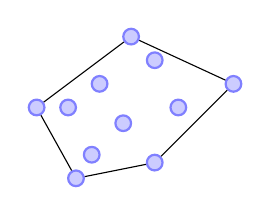
\begin{tikzpicture}[
          n/.style={circle,draw=blue!50,fill=blue!20,thick,inner sep=2pt}
          ]
          \node[n] (a) at (0,1.5)   {};
          \node[n] (b) at (1.2,2.4) {};
          \node[n] (c) at (2.5,1.8) {};
          \node[n] (d) at (1.5,0.8) {};
          \node[n] (e) at (0.5,0.6) {};
          \draw  (a) to (b) to (c) to (d) to (e) to (a);
          \node[n] at (1.5,2.1) {};
          \node[n] at (1.8,1.5) {};
          \node[n] at (1.1,1.3) {};
          \node[n] at (0.4,1.5) {};
          \node[n] at (0.8,1.8) {};
          \node[n] at (0.7,.9) {};
        \end{tikzpicture}       
      \end{column}
      \begin{column}{.75\linewidth}
        \begin{itemize}
        \item Sort points by x-coordinate, then y-coordinate
        \item Add them from left to right into the hull:
          \begin{itemize}
          \item New rightmost point is on the boundary
          \item Adding point to boundary may cause others to be deleted\\
            {\small depending on whether the angle is convex or not}
          \end{itemize}
        \end{itemize}
      \end{column}
    \end{columns}
  \end{block}

  \begin{block}{Huffman codes}
    \begin{itemize}
    \item When storing a text, giving each letter's code the same length wastes
      space
    \item \structure{Example:} $e$ is more common than $q$, so give it a
      shorter code
    \item \structure{Huffman encoding:} Sort letters by frequency, assign codes
      in order
    \end{itemize}
    \begin{columns}
      \begin{column}{.3\linewidth}
        \begin{tabular}{|c|c|l|}\hline
          Char&Freq.&Code\\\hline
          f&5&1100\\
          e&6&1101\\
          c&12&100\\\hline
        \end{tabular}        
      \end{column}
      \begin{column}{.3\linewidth}
        \begin{tabular}{|c|c|l|}\hline
          Char&Freq.&Code\\\hline
          b&13&101\\
          d&16&111\\
          a&45&0\\\hline
        \end{tabular}
      \end{column}
      \begin{column}{.35\linewidth}
        \begin{itemize}
        \item Simple \& fast
        \item Not best compression
        \item Used in JPEG and MP3
        \end{itemize}
      \end{column}
    \end{columns}
  \end{block}
\end{frame}
%%%%%%%%%%%%%%%%%%%%%%%%%%%%%%%%%%%%%%%%%%%%%%%%%%%%%%%%%%%%%%%%%%%%%%%%%%%%%%
\subsubsection{MergeSort}
\begin{frame}{Merge Sort}
  \begin{block}{Recursive sorting}
    \begin{itemize}
    \item Imagine the simpler way to sort recursively a list
    \visible<2->{
    \item[1.] Split your list in two sub-lists\\
      \visible<3->{\small One idea is to split evenly, but not the only one}
    \item[2.] Sort each of them recursively\\
      \visible<3->{\small (base case: size$\leq$1)}
    \item[3.] Merge sorted sublists back\\
      \visible<3->{\small at each step, pick smallest remaining elements of
        sublists, put it after already picked}
    }
    \end{itemize}
  \end{block}

  \begin{columns}
    \begin{column}{.55\linewidth}
      \begin{block}<4->{Merge Sort}
        \begin{itemize}
        \item List splited evenly
        \item Sub-list copied away
        \item Merge trivial
        \end{itemize}        
        (invented by John von Neumann in 1945)
      \end{block}      
    \end{column}
    \begin{column}{.4\linewidth}
      \visible<4->{\includegraphics{fig/sort_merge.fig}}
    \end{column}
  \end{columns}
\end{frame}
%%%%%%%%%%%%%%%%%%%%%%%%%%%%%%%%%%%%%%%%%%%%%%%%%%%%%%%%%%%%%%%%%%%%%%%%%% 
\begin{frame}[fragile]{Merge Sort}
  \begin{block}{Scala code}\smallskip
    \begin{columns}
      \begin{column}{.45\linewidth}
        \begin{boitecode}{}
def mergeSort(m: List[Int]):List[Int] =\{
  \structure{// short enought to be already sorted}
  if (m.length <= 1) 
    return m

  \structure{// Slice (=cut) the array in two parts}
  val middle = m.length / 2
  val left  = m.slice(0,middle)
  val right = m.slice(middle,m.length)
  
  \structure{// Sort each parts}
  val leftSorted  = mergeSort(left)
  val rightSorted = mergeSort(right)

  \structure{// Merge them back}
  return merge(leftSorted, rightSorted)
\}          
        \end{boitecode}
%        \vspace{-.8\baselineskip}{\tiny~~ (C) Wikipedia}
      \end{column}
      \begin{column}{.4\linewidth}
        \begin{boitecode}{}
def merge(xs:List[Int], ys:List[Int]) 
    :List[Int] = \{

  (xs,ys) match \{

    case ( _ , Nil) => xs
    case (Nil,  _ ) => ys

    case (x::x2, y::y2) =>
       if (x < y) \{
          x :: merge(x2 , ys)
       \} else \{
          y :: merge(xs , y2)
       \}
  \}
\}
        \end{boitecode}
      \end{column}
    \end{columns}
  \end{block}
  \begin{block}{Complexity Analysis}
    \begin{itemize}
    \item \structure{Time:} $\log(n)$ recursive calls, each of them being
      linear $\leadsto \alert{\Theta(n\times \log(n))}$
    \item \structure{Space:} Need to copy the array $\leadsto 2n$ (quite
      annoying) + $log(n)$ for the stack
    \end{itemize}
  \end{block}
\end{frame}
%%%%%%%%%%%%%%%%%%%%%%%%%%%%%%%%%%%%%%%%%%%%%%%%%%%%%%%%%%%%%%%%%%%%%%%%%% 
\subsubsection{QuickSort}
%%%%%%%%%%%%%%%%%%%%%%%%%%%%%%%%%%%%%%%%%%%%%%%%%%%%%%%%%%%%%%%%%%%%%%%%%% 
\begin{frame}{QuickSort}

  \begin{block}{Presentation}
    \begin{itemize}
    \item Invented by C.A.R. Hoare in 1962
    \item Widely used (in C library for example)
    \end{itemize}
  \end{block}

  \begin{block}{Big lines}
    \begin{itemize}
    \item Pick one element, called \alert{\textit{pivot}}
      (random is ok)
    \item Reorder elements so that:
      \begin{minipage}{.55\linewidth}
        \begin{itemize}
        \item elements smaller to the pivot are before it%
          \vspace{-.4\baselineskip}
        \item elements larger to the pivot are after it
        \end{itemize}
      \end{minipage}
    \item Recursively sort the parts before and after the pivot
    \end{itemize}
  \end{block}

  \begin{block}{Questions to answer}
    \begin{itemize}
    \item How to pick the pivot? (random is ok)
    \item How to reorder the elements?
      \begin{itemize}
      \item \structure{First solution:} build sub-list (but this requires extra
        space)
      \item \structure{Other solution:} invert in place (but hinders stability,
        see below)
      \end{itemize}
    \end{itemize}
  \end{block}
\end{frame}
%%%%%%%%%%%%%%%%%%%%%%%%%%%%%%%%%%%%%%%%%%%%%%%%%%%%%%%%%%%%%%%%%%%%%%%%%% 
\begin{frame}[fragile]{Simple Quick Sort}
  \begin{columns}
    \begin{column}{.44\linewidth}
      \begin{block}{It's easy with sub-lists:}
        \begin{itemize}
        \item Create two empty list variables
        \item Iterate over the original list;
          copy elements in correct sublist
        \item Recurse
        \item Concatenate results
        \end{itemize}
      \end{block}
    \end{column}
    \begin{column}{.55\linewidth}
    \begin{boitecode}{}
def quicksort(lst:List[Int]):List[Int] = \{
  if (lst.length <= 1) \structure{// Base case}
    return lst
  
  \structure{// Randomly pick a pivot value}
  val pivot = lst(lst.length / 2)      

  \structure{// split the list}
  var lows: List[Int] = Nil
  var mids: List[Int] = Nil
  var highs: List[Int] = Nil
  for (item <- lst) \{ \structure{// classify the items}
    if ( item == pivot)    \{ mids  = item :: mids \}
    else if (item < pivot) \{ lows  = item :: lows \}
    else                   \{ highs = item :: highs\}
  \}

  \structure{// return sorted list appending chunks}
  quicksort(lows) ::: mids ::: quicksort(highs) 
\}      
    \end{boitecode}      
    \end{column}
  \end{columns}

  \begin{block}{Problem}
    \begin{itemize}
    \item Space complexity is about $2n+\log(n))$...\\
      {\small (2n for array duplication, log(n) for the recursion stack)}
    \end{itemize}
  \end{block}
\end{frame}
%%%%%%%%%%%%%%%%%%%%%%%%%%%%%%%%%%%%%%%%%%%%%%%%%%%%%%%%%%%%%%%%%%%%%%%%%% 
\begin{frame}[fragile]{In-place Quick Sort}
  \null\vspace{-2.3\baselineskip}
  \begin{columns}
    \begin{column}{.6\linewidth}
      \begin{block}{Big lines of the list reordering}
        \begin{itemize}
        \item Put the pivot at the end
        \item Traverse the list
          \begin{itemize}
          \item If visited element is larger, do nothing
          \item Else swap with ``storage point'' \\
            + shift storage right
          \item[] (storage point is on left initially)
          \end{itemize}
        \item Swap pivot with storage point
        \end{itemize}
      \end{block}      
    \end{column}
    \begin{column}{.4\linewidth}
      \includegraphics{fig/sort_qsort.fig}      
    \end{column}
  \end{columns}\vspace{-.8\baselineskip}

  \begin{center}
    \begin{boitecode}{}
def quicksort(array:Array[Int]) \{
  def lambda(array:Array[Int], left:Int, right:Int, pivotIndex:Int) \{
    val pivotValue = array(pivotIndex)
    array.swap(pivotIndex, right) \structure{// Move pivot to end (swap() does not exist)}
    val storeIndex = left
    for (i <- left to right-1) \{
      if (array(i) <= pivotValue) \{
        array.swap(i, storeIndex)
        storeIndex = storeIndex + 1
    \} \}
    array.swap(storeIndex, right) \structure{// Move pivot to its final place}
    lambda(array, left, pivotIndex, (pivotIndex-left)/2)
    lambda(array, pivotIndex, right, (right-pivotIndex)/2)
  \}
  lambda(array, 0, array.length-1, array.length/2) \}
  \end{boitecode}
 \end{center}
\end{frame}
%%%%%%%%%%%%%%%%%%%%%%%%%%%%%%%%%%%%%%%%%%%%%%%%%%%%%%%%%%%%%%%%%%%%%%%%%%%%%
\begin{frame}{In-place QuickSort Complexity (1/2)}
  
  \begin{block}{Best case for divide-and-conquer algorithms: \alert{Even Split}}
    \begin{itemize}
    \item Split the amount of work by 2 at each step (thus $\Theta(log(n))$
      recursive calls)
    \item Work on each subproblem linear with its size (thus each call in
      $\Theta(n)$)
    \end{itemize}
  \end{block}

  \begin{block}{The recursion tree for best case:}\medskip
    \centerline{
      \includegraphics[width=.7\linewidth]{fig/algo_quick_bestcase.fig}
    }
  \end{block}

  \begin{block}{What if we split 1\%/99\% at each step (instead of 50\%/50\%)?}
    \begin{itemize}
    \item We get \visible<2->{$100\times\log(n)$} steps 
          $\leadsto$ whole algorithm in \visible<3->{$\Theta(n\log(n))$}
    \end{itemize}
  \end{block}
\end{frame}
%%%%%%%%%%%%%%%%%%%%%%%%%%%%%%%%%%%%%%%%%%%%%%%%%%%%%%%%%%%%%%%%%%%%%%%%%%%%%
\begin{frame}{In-place QuickSort Complexity (2/2)}
  \begin{block}{What if we have a fixed amount on one side?}
    \begin{itemize}
    \item (happens when every values are duplicated, or with the wrong pivot)

    \centerline{
      \includegraphics[width=.6\linewidth]{fig/algo_quick_worstcase.fig}
    }
    \item We get \visible<2->{$O(n)$} steps 
      $\leadsto$ whole algorithm in \visible<3->{\alert{$O(n^2)$}} in worst case
    \end{itemize}    
  \end{block}\vspace{-.4\baselineskip}

  \begin{block}{That's a fairly bad worst case time}
    \begin{itemize}
    \item Worst than MergeSort, for example
    \item But called Quicksort anyway because faster \textit{in practice}
      than MergeSort% and HeapSort
    \item In-Place version of both algorithms are \alert{not stable}
    \item Both can be quite easily parallelized
    \item \structure{Space complexity:}
      $O(\log(n))$ (to store the recursion stack)
    \end{itemize}
  \end{block}\vspace{-\baselineskip}

  \begin{flushright}
    (this ends the second lecture)    
  \end{flushright}
\end{frame}
%%%%%%%%%%%%%%%%%%%%%%%%%%%%%%%%%%%%%%%%%%%%%%%%%%%%%%%%%%%%%%%%%%%%%%%%%%%%%%

%%% Local Variables:
%%% coding: utf-8
